\documentclass{article}

\usepackage{graphicx}

\usepackage{amsfonts}
\usepackage{amssymb}
\usepackage{amsmath}
\usepackage{multicol}
\usepackage{xcolor}

\usepackage{tikz}
\usetikzlibrary{angles, quotes}

\graphicspath{ {fisica-generale/assets/} }

\begin{document}

\section{Cinematica}

La cinematica è lo studio moto. Il moto dipende dal sistema di riferimento.

\begin{center}
\begin{tikzpicture}
\coordinate (O) at (0,0,0);
\coordinate (p) at (2,2,0);
\coordinate (r) at (4,2,0);

\draw[ultra thick,black,->] (O) -- (7,0,0) coordinate(y) node[right]{y};
\draw[ultra thick,black,->] (O) -- (0,4,0) coordinate(z) node[above]{z};
\draw[ultra thick,black,->] (O) -- (0,0,4) coordinate(x) node[below]{x};

\draw[thick,blue,->] (O) -- (r) coordinate(r_t) node[midway,below,sloped]{$\vec{r}(t)$};

\filldraw[cyan] (p) circle(1.5pt) node[below]{p};
\draw[thick,cyan] plot [smooth] coordinates {(p) (3,2.5,0) (r) (5,1.5,0) (6,2,0)};
\end{tikzpicture}
\end{center}

\noindent
Possiamo descrivere il moto di un punto materiale come una funzione.

$$
\begin{matrix}
r: &\mathbb{R} &\to &\mathbb{R}^3 \\
&t &\to &\vec{r}(t)
\end{matrix}
$$

\subsection{Punto}

\subsubsection{Definizione}

Dato $\vec{r}(t)$ che descrive il moto di un punto, definiamo la traiettoria come il luogo dei punti dello spazio "esplorati" da $\vec{r}(t)$ al variare di $t$.

\noindent
$\vec{r}(t)$ è un vettore dimensionale:

$$
\vec{r}(t) = (r_x(t), r_y(t), r_z(t))
$$

\subsubsection{Notazione}

$$
[r_x] = (m)
$$

\subsection{Velocità}

\subsubsection{Definizione}

La velocità è una funzione vettoriale che associa ad ogni tempo "lo spostamento infinitesimo" in un intervallo di tempo infinitesimo.

\begin{center}
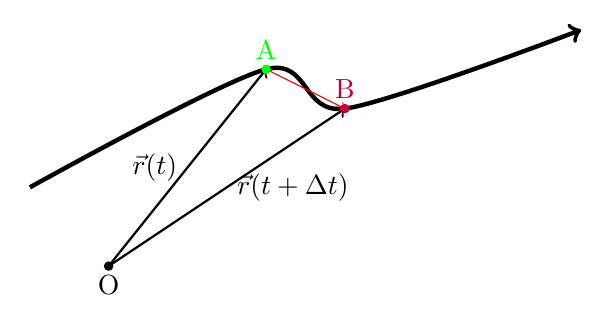
\begin{tikzpicture}
\coordinate (O) at (0,0);
\coordinate (p) at (-1,1);
\coordinate (A) at (2,2.5);
\coordinate (B) at (3,2);

\draw[ultra thick,black,->] plot [smooth] coordinates {(p) (A) (B) (6,3)};
\draw[thick,black,->] (O) -- (A) node[midway,left]{$\vec{r}(t)$};
\draw[thick,black,->] (O) -- (B) node[midway,right]{$\vec{r}(t + \Delta t)$};
\draw[red,->] (A) -- (B);

\filldraw[black] (O) circle(1.5pt) node[below]{O};
\filldraw[green] (A) circle(1.5pt) node[above]{A};
\filldraw[purple] (B) circle(1.5pt) node[above]{B};
\end{tikzpicture}
\end{center}

$$
\vec{v}(t) = \lim_{\Delta t \to 0} \frac{\vec{r}(t + \Delta t) - \vec{r}(t)}{\Delta t} = \frac{d}{dt} \vec{r}(t)
$$

\noindent
$\vec{v}(t)$ è un vettore che possiamo esprimere in componenti

$$
\vec{v}(t) = (v_x(t), v_y(t), v_z(t))
$$

\noindent
Perciò:

$$
\begin{matrix}
\vec{r}(t) = (r_x(t), r_y(t), r_z(t)) \\
v_x(t) = \frac{d}{dt} r_x(t) \\
v_y(t) = \frac{d}{dt} r_y(t) \\
v_z(t) = \frac{d}{dt} r_z(t)
\end{matrix}
$$

\subsubsection{Notazione}

La velocità si misura in $m/s$

\subsubsection{Proprietà della derivata}

\begin{itemize}
    \item $\frac{d}{dt}(\vec{f}(t) + \vec{g}(t)) = \frac{d}{dt}\vec{f}(t) + \frac{d}{dt}\vec{g}(t)$
    \item Sia $\lambda(t)$ una funzione reale in $\mathbb{R}$ e $\vec{f}(t) \in \mathbb{R}^3$: $\frac{d}{dt}(\lambda(t)\vec{f}(t)) = (\frac{d}{dt}\lambda(t))\vec{f}(t) + \lambda(t)(\frac{d}{dt}\vec{f}(t))$
    \item Siano $\vec{f}(t), \vec{g}(t) \in \mathbb{R}^3$, allora: $\frac{d}{dt}(\vec{f}(t)\vec{g}(t)) = (\frac{d}{dt}\vec{f}(t))\vec{g}(t) + \vec{f}(t)(\frac{d}{dt}\vec{g}(t))$
    \item $\frac{d}{dt}(\vec{f}(t) \wedge \vec{g}(t)) = (\frac{d}{dt}\vec{f}(t)) \wedge \vec{g}(t) + \vec{f}(t) \wedge (\frac{d}{dt}\vec{g}(t))$
\end{itemize}

\subsection{Accelerazione}

\subsubsection{Definizione}

Dato $\vec{r}(t)$ con velocità $\vec{v}(t)$, definiamo l'accelerazione come:

$$
\vec{a}(t) = \lim_{\Delta t \to 0} \frac{\vec{v}(t + \Delta t) - \vec{v}(t)}{\Delta t} = \frac{d}{dt} \vec{v}(t) = \frac{d^2}{dt^2} \vec{r}(t)
$$

\noindent
Graficamente, la velocità è sempre tangente alla traiettoria.

\includegraphics[width=\columnwidth]{rappresentazione-accelerazione-grafica}

\noindent
Si può identificare graficamente l'accelerazione come differenza dei vettori $\vec{v}(t)$ e $\vec{v}(t + \Delta t)$ per $\Delta t$ "piccolo"

\includegraphics[width=\columnwidth]{rappresentazione-accelerazione-grafica-differenza}

\noindent
Perciò vale la formula (si usa $\simeq$ poiché $\Delta t$ è finito):

$$
\vec{a}(t) \simeq \frac{\vec{v}(t + \Delta t) - \vec{v}(t)}{\Delta t}
$$

\noindent
che graficamente è:

\includegraphics[width=\columnwidth]{rappresentazione-accelerazione-grafica-approssimazione}

\subsection{Il "problema inverso"}

Capita molto più spesso di avere informazioni su $\vec{v}(t)$ o $\vec{a}(t)$ e di voler ricostruire $\vec{r}(t)$. Questo è definito come il "problema inverso" della cinematica, che si riconduce alla risoluzione di equazioni differenziali

\end{document}
